\documentclass{article}
\usepackage[utf8x]{inputenc}
\usepackage{ucs}
\usepackage{amsmath} 
\usepackage{amsfonts}
\usepackage{upgreek}
\usepackage[english,russian]{babel}
\usepackage{graphicx}
\usepackage{float}
\usepackage{textcomp}
\usepackage{hyperref}
\usepackage{geometry}
  \geometry{left=2cm}
  \geometry{right=1.5cm}
  \geometry{top=1cm}
  \geometry{bottom=2cm}
\usepackage{tikz}
\usepackage{ccaption}
\usepackage{multicol}

\usepackage{listings}
%\setlength{\columnsep}{1.5cm}
%\setlength{\columnseprule}{0.2pt}


\begin{document}
\pagenumbering{gobble}

\lstset{
  language=C++,                % choose the language of the code
  basicstyle=\linespread{1.1}\ttfamily,
  columns=fixed,
  fontadjust=true,
  basewidth=0.5em,
  keywordstyle=\color{blue}\bfseries,
  commentstyle=\color{gray},
  stringstyle=\ttfamily\color{orange!50!black},
  showstringspaces=false,
  %numbers=false,                   % where to put the line-numbers
  numbersep=5pt,
  numberstyle=\tiny\color{black},
  numberfirstline=true,
  stepnumber=1,                   % the step between two line-numbers.        
  numbersep=10pt,                  % how far the line-numbers are from the code
  backgroundcolor=\color{white},  % choose the background color. You must add \usepackage{color}
  showstringspaces=false,         % underline spaces within strings
  captionpos=b,                   % sets the caption-position to bottom
  breaklines=true,                % sets automatic line breaking
  breakatwhitespace=true,         % sets if automatic breaks should only happen at whitespace
  xleftmargin=.2in,
  extendedchars=\true,
  keepspaces = true,
}
\lstset{literate=%
   *{0}{{{\color{red!20!violet}0}}}1
    {1}{{{\color{red!20!violet}1}}}1
    {2}{{{\color{red!20!violet}2}}}1
    {3}{{{\color{red!20!violet}3}}}1
    {4}{{{\color{red!20!violet}4}}}1
    {5}{{{\color{red!20!violet}5}}}1
    {6}{{{\color{red!20!violet}6}}}1
    {7}{{{\color{red!20!violet}7}}}1
    {8}{{{\color{red!20!violet}8}}}1
    {9}{{{\color{red!20!violet}9}}}1
}

\title{Задание: Паттерн Состояние. \vspace{-5ex}}\date{}\maketitle

\section*{Описание программы}
В папке \texttt{src} лежит исходный код программы, в которой используется паттерн Состояние для описания передвижения персонажа двумерной компьютерной игры. Персонаж может передвигаться по карте, при этом он может находиться в следующих состояниях:
\begin{itemize}
\item \texttt{Idle} -- стояние на месте
\item \texttt{Running} -- бег
\item \texttt{Falling} -- обычное падение. При прыжке (клавиша \texttt{Space}) персонаж переходит в это состояние.
\item \texttt{Sliding} -- скольжение. В это состояние можно перейти из состояния бега, нажав на клавишу левый \texttt{Shift}. По истечению некоторого времени, при условии, что персонаж касается земли, он переходит в состояние \texttt{Idle} или \texttt{Running}.
\item \texttt{Hooked} -- зацепление за край блока. В это состояние можно перейти из состоя \texttt{Falling} оказавись рядом с краем блока. Выйти из этого состояния можно подпрыгнув или нажав стрелочку вниз.
\end{itemize}

\subsection*{Класс \texttt{Animation}}
В программе используется спрайтовая анимация. Все возможные положения персонажа во всех состояниях хранятся в одном изображении \texttt{hero.png}. Эта текстура загружается в программу с помощью класса \texttt{sf::Texture}. В дальнейшем мы можем отрисовывать на экране любой прямоугольник из этой текстуры. Для удобства отрисовки этих прямоугольников на экран используется специальный объект класса \texttt{sf::Sprite}.
\begin{center}
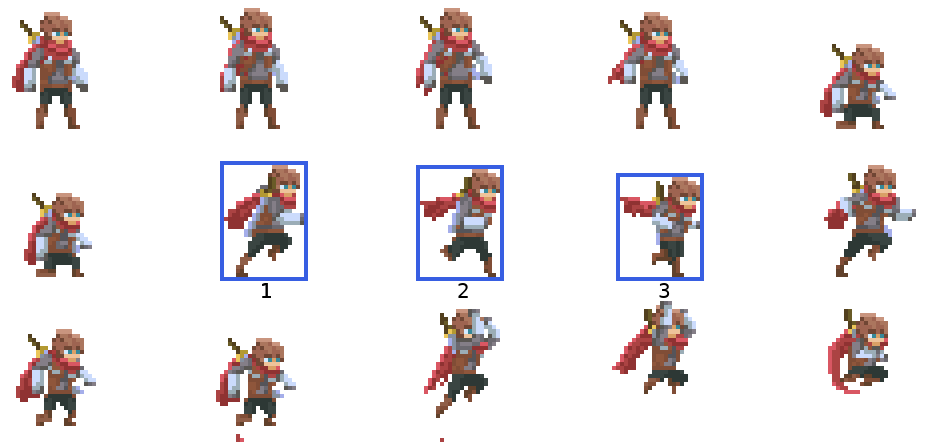
\includegraphics[scale=0.3]{../images/hero_texture_rects.png}
\end{center}
Например, для отрисовки бега персонажа сначала на месте персонажа рисуется изображение из прямоугольника \texttt{1} (смотрите рисунок), затем изображение из прямоугольника \texttt{2} и так далее.\\

Поля класса \texttt{Animation}:
\begin{itemize}
\item \texttt{mTextureRects} -- контейнер, который хранит в себе координаты всех прямоугольников данной анимации.
\item \texttt{mCurrentFrame} -- номер текущего кадра-прямоугольника из вектора \texttt{mTextureRects}.
\item \texttt{mAnimationSpeed} -- скорость анимации
\item \texttt{mTime} -- текущее время анимации
\item \texttt{mType} -- тип анимации. Может принимать следующие значения:
\begin{itemize}
\item \texttt{Animation::Repeat} -- анимация повторяется. Используется, например, для анимации бега персонажа.
\item \texttt{Animation::OneIteration} -- анимация проигрывается один раз, а затем застывается на последнем кадре. Используется для анимации скольжения и анимации зацепления за отвес.\\
\end{itemize}

Методы класса \texttt{Animation}:

\begin{itemize}
\item \texttt{void update(float dt)} -- Увеличивает время текущей анимации на \texttt{dt}. Может изменить текущий кадр анимации. Вызывается каждый кадр.
\item \texttt{void updateSprite(sf::Sprite\& sprite)} -- Устанавливает соответствующий прямоугольник текстуры для передаваемого спрайта.

\end{itemize}


\subsection*{Класс \texttt{Player}}
Поля класса \texttt{Player}:
\begin{itemize}
\item \texttt{mPosition} -- положение персонажа
\item \texttt{mVelocity} -- скорость персонажа
\item \texttt{mCollisionRect} -- прямоугольник, используемый для обнаружения столкновений персонажа с миром. Координаты прямоугольника отсчитываются от положения персонажа (\texttt{mPosition}).
\item \texttt{mIsColliding} -- переменная, которая показывает касается ли перонаж какого либо из блоков.
\item \texttt{mpState} -- указатель на состояние персонажа. Тут используется полиморфизм, чтобы менять состояние персонажа.
\item \texttt{mTexture} -- текстура
\item \texttt{mSprite} -- спрайт
\item \texttt{mScaleFactor} -- масштаб персонажа.
\item \texttt{mIsFacedRight} -- параметр, задающий направление персонажа.
\end{itemize}

Методы класса \texttt{Player}:
\begin{itemize}
\item \texttt{void update(float dt)} -- обновляем положение персонажа и анимацию на время \texttt{dt} вперёд.
\item \texttt{void draw(sf::RenderWindow\& window)} -- рисуем персонажа на окне.
\item \texttt{void handleEvents(const sf::Event\& event)} -- обрабатываем все события, связанные с персонажем.
\item \texttt{bool handleCollision(const sf::FloatRect\& rect)} -- проверяем столкновение персонажа и прямоугольника \texttt{rect}.
\item \texttt{void handleAllCollisions(const std::vector<sf::FloatRect>\& blocks)} -- проверяем столкновение персонажа с вектором из прямоугольников. Устанавливаем значение поля \texttt{mIsColliding}.
\end{itemize}


\subsection*{Класс \texttt{World}}
Поля класса \texttt{World}:
\begin{itemize}
\item \texttt{mBlocks} -- контейнер-вектор, который хранит в себе прямоугольки, описывающие карту мира.
\item \texttt{mPlayer} -- игрок.
\item \texttt{mGravity} -- сила гравитации.
\item \texttt{mView} -- вид. Объект специального класса \texttt{sf::View}, который позволяет удобно двигать камеру в 2-х измерениях.
\end{itemize}

Методы класса \texttt{World}:
\begin{itemize}
\item \texttt{void update(float dt)} -- обновляем мир на \texttt{dt} вперёд по времени.
\item \texttt{void setView()} -- устанавливаем камеру в зависимости от положения игрока.
\item \texttt{draw}, \texttt{handleEvents}, \texttt{addBlock}.

\end{itemize}
\newpage
\subsection*{Класс \texttt{PlayerState} и его наследники}
Состояния персонажа реализовано с помощью абстрактного класса \texttt{PlayerState} и его наследников -- классов описывающих каждое состояние: \texttt{Idle}, \texttt{Running}, \texttt{Falling}, \texttt{Sliding}, \texttt{Hooked}.

\texttt{PlayerState} хранит в себе анимацию(\texttt{mAnimation}) и силу прыжка (\texttt{kJumpingVelocity}) так как эти поля являются общими для всех классов. У этого класса также есть следующие абстрактные методы:

\begin{itemize}
\item \texttt{update} - метод, который вызывается каждый кадр.
\item \texttt{handleEvents} - метод, для обработки всех событий (например, нажатий клавиш). Срабатывает каждый кадр.

\item \texttt{startFalling} - метод, который срабатывает, когда персонаж перестаёт касаться земли. В этом случае, если мы находимся в состоянии \texttt{Running} или \texttt{Idle}, мы должны перейти в состояние \texttt{Falling}. В остальных случаях мы должны ничего не делать.
\item \texttt{hitGround} - метод, который срабатывает, когда персонаж касается земли. В этом случае, если мы находимся в состоянии \texttt{Falling}, мы должны перейти в состояние \texttt{Idle}. В остальных случаях мы должны ничего не делать.
\item \texttt{hook} - метод, который срабатывает, когда персонаж подходит близко к уступу. В этом случае, если мы находимся в состоянии \texttt{Falling}, мы должны перейти в состояние \texttt{Hooked}. В остальных случаях мы должны ничего не делать.
\end{itemize}

Эти абстрактные методы переопределяются в наследниках класса \texttt{PlayerState}. Благодаря такому полиморфизму и добивается удобное изменение состояний объекта. Так как указатель на состояние \texttt{mpState}, хранящийся в объекте класса \texttt{Player} может менять свой динамический тип и, соответственно, при вызове
\begin{lstlisting}
mpState->update(dt);
\end{lstlisting}
будет вызываться переопределённый виртуальный метод, соответствующий текущему состоянию.

\begin{center}
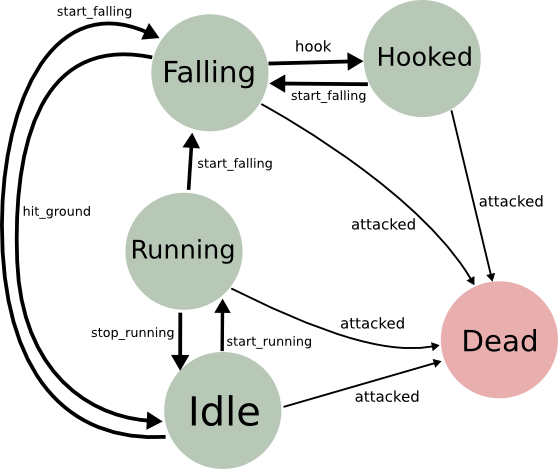
\includegraphics[scale=0.8]{../images/hero_fsm.png}
\end{center}


\end{itemize}

\newpage
\section*{Задачи}

\subsection*{Двойной прыжок}
Измените состояние \texttt{Falling}, добавив возможность совершения персонажем двойного прыжка. Если персонаж перешёл в состояние \texttt{Falling} прыгнув или упав с уступа он должен иметь возможность прыгнуть в воздухе ещё один раз. Сила второго прыжка должна быть меньше, чем сила первого.


\subsection*{Состояние сидения}
Добавьте новое состояние под названием \texttt{Sitting}. Персонаж должен переходить в это состояние из состояние \texttt{Idle} путём нажатия клавиши левый \texttt{Shift}.

\subsection*{Состояние атаки}
Добавьте новые состояния для атаки персонажа. При нажатии на клавишу \texttt{X}, если персонаж находится в состояниях \texttt{Idle} или \texttt{Running}, он должен начать атаку и перейти в состояние \texttt{FirstAttack}.

\begin{center}
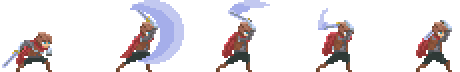
\includegraphics[scale=0.7]{../images/hero_texture_attack.png}
\end{center}

После завершения первой атаки, если пользователь не нажимает клавишу \texttt{X}, то персонаж должен перейти в состояние \texttt{Idle}. Если же во время первой атаки пользователь ещё раз нажал клавишу \texttt{X}, то персонаж, по окончанию анимации, должен перейти из состояния \texttt{FirstAttack} в состояние \texttt{SecondAttack}.
\begin{center}
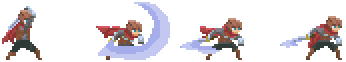
\includegraphics[scale=0.7]{../images/hero_texture_attack2.png}
\end{center}

После завершения второй атаки, если пользователь не нажимает клавишу \texttt{X}, то персонаж должен перейти в состояние \texttt{Idle}. Если же во время второй атаки пользователь ещё раз нажал клавишу \texttt{X}, то персонаж, по окончанию анимации, должен перейти из состояния \texttt{SecondAttack} в состояние \texttt{ThirdAttack}.
\begin{center}
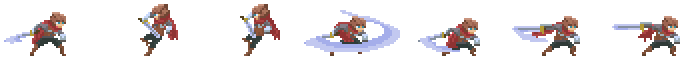
\includegraphics[scale=0.7]{../images/hero_texture_attack3.png}
\end{center}

По окончанию третьей атаки персонаж должен перейти в состояние \texttt{Idle}. Если персонаж на момент начала атаки находился в состоянии \texttt{Running}, то он не должен мгновенно терять скорость. Скорость персонажа, полученная в состоянии \texttt{Running} должна плавно затухать во время проведения атак. 

Анимацию атак можно посмотреть в файле \texttt{attack.gif}.


\subsection*{Разрушаемые объекты}
Добавьте на карту объекты, которые можно будет разрушать. В качестве объектов можно взять просто круги, при разрушении они должны исчезать. Объекты должны разрушаться только в момент проведения атаки и только если они касаются или оказываются близко к мечу персонажа.

\end{document}